\documentclass[twocolumn]{article}
\usepackage{cite,tikz}
%\usepackage{algorithm,algpseudocode}
\usepackage[margin=1in]{geometry}
\usepackage{url,graphicx}
\usetikzlibrary{shapes, calc} 
\tikzstyle{vertex}=[draw,fill=black!15,circle,minimum size=20pt,inner sep=0pt]
\title{Cluster-Based Analysis for\\Combatting DDoS Attacks}
\author{Bryan Cuccioli}
\date{Cornell University}
\begin{document}
\maketitle

\begin{abstract}
\emph{Distributed denial of service attacks constitute one of the most easily exploited and difficult to defend against risks to computer network security. We propose a route-based system for recognizing and mitigating DDoS attacks as they occur in real time. The system is designed with the primary goal of recognizing requests from illegitimate sources participating in a DDoS attack using time-based sequential k-means clustering, enabling the service to drop those requests while still handling and performantly responding to those representing legitimate users.}

\emph{We implement the proposed design for a simplified use case in Java. We find that with the classifying gateway in place, the average latency of the service does not increase past the standard error margin when the system is exposed to multiple other hosts continuously sending requests.}
\end{abstract}

\section{Introduction}

Distributed denial of service (DDoS) attacks are among the most common, devastating, and difficult to prevent security risks facing the Internet today. Such attacks consist generally of flooding a target service with a sufficiently high number of requests as to take processing time for legitimate requests, introduce instability into the system, and surface latent issues with the service that are only visible at large scale. Attackers are able to carry out DDoS attacks with large number of hosts under their control -- organized into so-called \emph{botnets} -- or in some cases with a small number of hosts that can cause other services to output large amounts of information, as in the case of \emph{DNS amplification} attacks.

DDoS attacks are particularly difficult to defend against because unlike most other computer security attacks, they are not dependent on and do not target specific vulnerabilities, either at the implementation level or protocol level. Rather, they are indistinguisable from legitimate user requests and traffic, except for their frequency. This has made quickly identifying and defending against DDoS attacks without interrupting the entire network service very difficult.

The goal of this project is to equip web services with a way to defend against DDoS attacks as easily and quickly as possible, with minimal disruption to the user experience. This mechanism should be completely transparent to the legitimate end-user, avoiding modifying their experience or the service's interface in the event of a DDoS attack. It should also be mostly transparent to the web service itself, requiring minimal feedback and overhead from the service so as to minimize the amount of extra processing power needed during a DDoS attack. Finally, this mechanism should not rely on extensive infrastructure modifications or those outside the control of the owner of the web service. Such modifications would require widespread adoption to work, and it would be difficult for the average service operator to have them implemented.

The design of this mechanism revolves around a network of gateway-like nodes between the web service and the rest of the Internet. These gateways will be responsible for distributing requests to the nodes of the service, using clustering techniques from machine learning to attempt to quickly separate legitimate hosts from those participating in the DDoS attack, silently discarding malicious requests and passing others on to the web service. This way, while the service will have to respond to some initial small number of malicious requests, it will be largely shielded from devoting processing power to them.

The remainder of this paper is as follows. In section 2, we discuss related work and how it compares with our proposal. In section 3, we give a detailed design overview for our system. In section 4, we give a more low-level overview of our implementation of the system. Finally, in section 5, we present our evaluation plan and empirical results, demonstrating the efficacy of the system.

\section{Related Work}

Because of the important security implications, a lot of work has already been done in this area using a variety of ideas derived from a number of differing perspectives. Below, we present a comprehensive cross-section of the techniques being researched and employed to prevent, protect against, and mitigate DDoS attacks.

\subsection{Friction-Based Prevention}

Some of the most basic ideas for mitigating DDoS attacks are based on a redesign at the level of the protocols governing network communications. In \emph{DoS: Fighting Fire with Fire} \cite{fire}, the authors propose limiting the rate of incoming requests and requiring users to aggressively retransmit their requests until they go through successfully; this is a version of the idea of requiring users to make micropayments to use the service, where the payments here come in the form of bandwidth.

Along a similar vein, the paper \emph{Game-Based Analysis of Denial-of-Service Prevention Protocols} \cite{game} proposes requiring the client to participate in a key exchange with the server before the server is able to handle any of its requests. This requires a micropayment in the form of client processing time, and has the added benefit of ensuring that the client is not spoofing the origin of their data. A very similar approach is taken in the paper \emph{Efficient, DoS-Resistant, Secure Key Exchange for Internet Protocols} \cite{key}.

\subsection{Route-Based Filtering}

Other researchers have been more focused on designing and implementing systems to perform route-based filtering, similar to our proposal. The paper \emph{On the Effectiveness of Route-Based Packet Filtering for Distributed DoS Attack Prevention in Power-Law Internets} \cite{power} discusses how effective certain techniques are for router-based packet filtering based on the assumption that the Internet obeys certain mathematical power law relationships with respect to the connectivities and degrees of its nodes. A similar approach is taken in the paper \emph{Mayday: Distributed Filtering for Internet Services} \cite{mayday}. In addition, the paper \emph{Using Active Networking to Thwart Distributed Denial of Service Attacks} \cite{active} uses a software-based network infrastructure called Active Networking which can be easily reprogrammed and reshaped to minimize the illegitimate traffic's effects on the service. While these systems all use route-based filtering, they differ from our system in that they use certain mathematical assumptions about the structure of the network rather than an adaptive, learning-based solution.

\subsection{Learning-Based Prevention}

Some have adapted principles from data mining and machine learning to the problem of DDoS recognition and prevention. Some of these techniques draw from the mathematical disciplines of probability and statistics. The paper \emph{Detecting DoS and DDoS Attacks by Using an Intrusion Detection System and Remote Prevention System} \cite{intrusion} uses a \emph{cumulative sum algorithm} from statistical quality control to determine whether a group of packets is from a DDoS attack. The paper \emph{Random Flow Network Modeling and Simulations for DDoS Attack Mitigation} \cite{flow} takes a more theoretical approach, constructing models based on network flow and running simulations based on idealized Internet topological models to analyse the emergent behaviour of DDoS attacks.

While these systems are based on learning techniques to help detect DDoS attacks, they are heavily theoretical and do not make much attempt to implement these ideas in practice. They use more complex mathematical models that may not be easily integrated into an existing system. Moreover, they do not break down the time-based data into dimensions reflecting normal operation versus operation under a DDoS attack.

\subsection{Traceback-Based Prevention}

One of the most useful changes in infrastructure to allow recognizing and defending against DDoS attacks would be the ability to trace a connection back to its source, mapping out the path it took to arrive at the target. One approach, taken in the paper \emph{Research on Authentication Scheme for DDoS Attack Source Traceback} \cite{auth} uses the \emph{reflection relay algorithm} and algebraic coding theory to mark packets and perform path reconstruction. The paper \emph{Reverse Traceroute} \cite{traceroute} describes the implementation of a system for similarly reconstructing the path a given packet took to arrive from its original source. The paper \emph{Network Support for IP Traceback} \cite{traceback} describes a novel approach towards achieving this capability without necessitating infrastructure modifications. This works by probabalistically marking packets and using a large number of them to reconstruct partial paths.


\begin{figure*}
\begin{center}

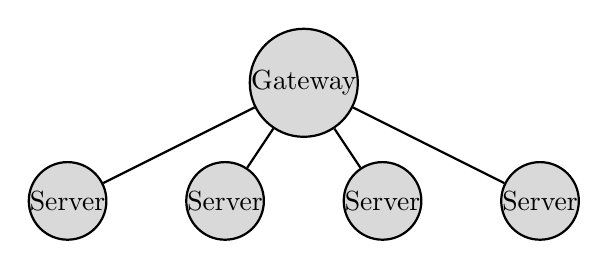
\begin{tikzpicture}[thick,level/.style={sibling distance=20mm/#1}]
\node[vertex] {Gateway}
  child { node[vertex] {Server} }
  child { node[vertex] {Server} }
  child { node[vertex] {Server} }
  child { node[vertex] {Server} };
\end{tikzpicture}
\end{center}
\caption{Topology of our system}
\label{fig:designtopology}
\end{figure*}

\section{Design}

We structure our system as a gateway guarding the nodes comprising the web service (Figure~\ref{fig:designtopology}). A larger or more sophisticated system may desire to partition the nodes behind multiple gateways linked to a load-balancing router. The gateway is responsible for enforcing a sharp upper bound on the rate of requests that get through to the web service for processing.

One of the central design tenets of our system is simplicity. The difficulty of implementing other anti-DDoS schemes has been a barrier to their adoption in practice. A system that is effective yet simple to integrate is more likely to be of use to administrators of web services.

\subsection{Routing}

For the sake of simplicity, the gateway performs simple routing of requests to each hosts in a round-robin-like fashion, based on the most recently reported load of the host. This load balancing scheme is furnished by the servers periodically communicating to the gateway information about what level of stress they are currently under. Each server $i$ re-calculates a \emph{load score} $L_i$. This embodies
\begin{enumerate}
\item the number of threads currently dispatched from their thread pools $T_i$ to handle requests, and
\item for each thread $t_j$, the amount of time $N_t$ the most recent request for the thread required to complete.
\end{enumerate}
In particular
\begin{equation}L_i=\sum_{t\in T_i} N_t.\end{equation}
This heuristic is intentionally simple: it provides a reasonable snapshot of the amount of load server $i$ is under without requiring too much processing power, and hence behaving as transparently as possible while also not appreciably skewing the actual load of the server.

Each gateway maintains a priority queue $P_j$ holding the servers (the \emph{server queue}), subject to the invariant that if $L_i<L_k$ for the most recently received values of $L_i$ and $L_k$, then $k\prec i$ in the priority queue. That is, a server has higher priority in the queue if its load score is lower. Moreover, there is a user-defined \emph{load threshold} $M$ that bounds above the amount of load a server can be under for it to be considered available. Explicitly, we do not add $i$ to $P_j$ if $L_i>M$ in the most recent update cycle.

In order to safely implement request dispatch, the gateway maintains a simple \emph{request queue} $Q_j$ of incoming requests. If $P_j$ is non-empty, the gateway immediately dequeues a server $i$ from $P_j$ and dispatches the incoming request to server $i$. Otherwise, the request is added to $Q_j$. After every update cycle, the gateway checks $P_j$ for a server, and if it finds one, dispatches the request to the server as described above.

\subsection{Request Classification}

The primary function of the gateway is to classify requests into two types: legitimate and malicious. We seek to perform the classification based on the relative times at which requests are seen. To this end, there are two dimensions of data we wish to measure: time and frequency of requests seen during normal operation; and time and frequency of requests seen when under a DDoS attack. This suggests using a cluster-based analysis to discern sources associated with normal operation from those associated with a DDoS attack.

Additionally, there are several necessary features for the classification process which we base our design around.

\begin{figure*}
\begin{center}
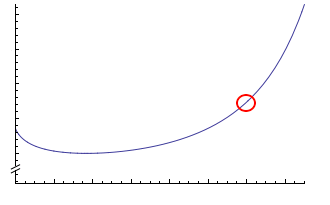
\includegraphics[width=5cm]{sim.png}
\end{center}
\caption{Illustration of the beginning of a DDoS event}
\label{fig:requests}
\end{figure*}

\begin{enumerate}
\item The classifier should mark request sources as malicious without having to see them a large number of times. Each time a classifier sees a request from a source and has not yet marked it as malicious, it will take up server processing time. 

\item The classifier should over time lower its confidence that the source is malicious if no further attacks occur. This is necessary in the event that the source IP address is leased to a legitimate host or in the event that the attacker has hijacked a host that would be sending legitimate requests and is using it as a zombie. The relative likelihood of these events is fairly low, so slowly lowering the confidence level that a source is malicious is acceptable.

\item Symmetrically, the classifier should slowly lower its confidence that the source is legitimate if no new DDoS event occurs, for the same reasons.
\end{enumerate}

With the above needs in mind, maintain a global coordinate plane which will hold unique request sources. When the service is not known to be experiencing a DDoS attack, we add the source of each incoming request to the plane with coordinates $(\alpha,\alpha)$ that it is a legitimate source. At each time interval $\tau$, we update $\alpha$ to $\alpha-\Delta\alpha$ for some small pre-defined value of $\Delta\alpha>0$. This encodes requirement (3) above.

We also globally track the rate of incoming requests at the gateway level. At every pre-defined interval $\tau$, we store $F(t)$: the number of requests that have been processed at time $t$. We also globally store the \emph{linearized derivative}
\begin{equation}\partial F(t)\approx \frac{F(t)-F(t-\tau)}{\tau}\end{equation}
and \emph{linearized second derivative}
\begin{equation}\partial^2 F(t)\approx 2\frac{F(t)-F(t-\tau)-\partial F(t-\tau)\cdot \tau}{\tau^2}.\end{equation}
(These are derived by interpolating $F$ to a continuous function and computing its first- and second-order Taylor series.)

These heuristics give a precise measurement of when the rate of requests is sharply increasing. When $F(t)$, $\partial F(t)$, and $\partial^2 F(t)$ rise above certain pre-defined thresholds, we say a DDoS event has begun at time $t$ (see Figure~\ref{fig:requests} for a possible illustration of the beginning of such an event, as recognized by the above heuristic). As new requests come in, we mark those requests with coordinates $(\beta,\beta)$. As above, after every time interval $\tau$, we decrease the confidence with which we believe a source to be malicious by $\Delta\beta$. This serves two purposes: it encodes requirement (2); and it biases malicious classification towards sources actually participating in the DDoS attack, since those sources are expected to send requests multiple times in fast succession.

When adding sources to the plane, we continuously perform a \emph{sequential k-means clustering} algorithm using a low-pass filter (Figure~\ref{fig:kmeans}). This algorithm is desirable because of its \emph{forgetful} property: newer samples receive more weight than older samples. More precisely, we can see that each mean reaches its final state in terms of its nearest samples as
\begin{equation}\mathbf{m}_i=\lambda\sum_{k=1}^n (1-\lambda)^{n-k} x_k.\end{equation}
This helps to encode properties (2) and (3). Moreover, the update step of the algorithm is very simple and can be implemented in only a few operations, minimizing the bottleneck effect of the classifier.

\begin{figure*}
\begin{center}
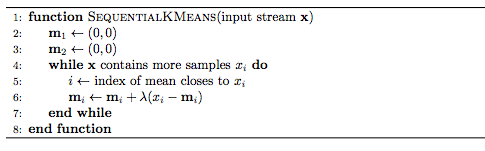
\includegraphics[width=10cm]{algo.png}
\end{center}
\caption{Sequential k-means clustering algorithm}
\label{fig:kmeans}
\end{figure*}

The end result of the above classification steps is we now have a strong notion of which sources are legitimate and which are actively participating in the DDoS attack against the web service. For example, the resulting clustering from a small-scale run is shown in Figure~\ref{fig:plane}. Now, when a gateway node receives a request, it first consults the classifier to determine whether the source is believed to be malicious. If the source has been classified as malicious with sufficiently high confidence, the gateway node simply resets the connection and discards the request. Otherwise, it adds the request to the request queue $Q_j$ as described above.

\begin{figure*}
\begin{center}
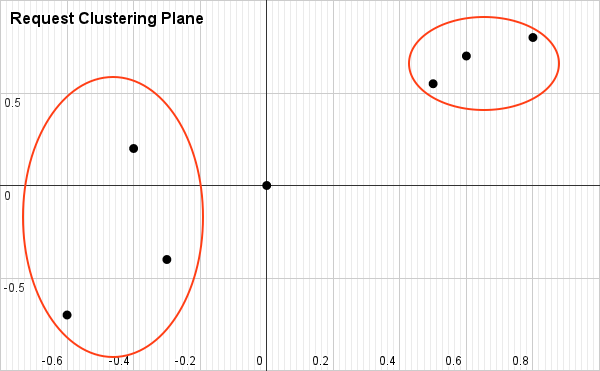
\includegraphics[width=8cm]{plane.png}
\end{center}
\caption{Sample clustering of requests}
\label{fig:plane}
\end{figure*}

\section{Implementation}

For the sake of quickly prototyping the system, we implement the system using Java. We will use the implementations included in the Java standard library for concurrency, socket communications, and the necessary data structures. 

\subsection{High-Level Implementation}

The class \texttt{Host} represents an abstraction for each server node in the system. Each \texttt{Host} instance has a load score, associated socket for communicating with the gateway, and a \texttt{Queue<Socket>} of incoming requests, the latter of which is not cached at the thread level. When writing a response back to the gateway, the \texttt{Host} also encodes the most recent load score in the response. Each thread running on a \texttt{Host} object repeatedly polls the queue for incoming requests, sends it to the server, reads the response, and writes the response back to the gateway.

Configuration variables are stored in a global static \texttt{Configuration} class as public static constants. This helps to easily expose the configuration settings and make the system easily tunable.

The \texttt{Clustering} class maintains a static \texttt{HashMap} which maps request sources to coordinates in the clustering plane, as well as a \texttt{BlockingQueue} of incoming samples to classify and current means for both clusters. It continuously polls the \texttt{BlockingQueue} for a new sample, at which point it updates its values in the \texttt{HashMap} and then updates the means accordingly -- this entire operation runs in $O(1)$ constant time to reduce the latency caused by the classifier. It exports a public function \texttt{isGoodHost(String)} which tells in $O(1)$ time to which cluster the given host belongs.

The entry point for the application is the \texttt{Gateway} class, which represents the routing gateway guarding the server nodes. This class maintains a \texttt{PriorityQueue<Host>} of \texttt{Host} objects, sorted by lowest recent load score. It also maintains a global request count and request derivatives. A special thread is forked for the \texttt{Updater} class, which is responsible for continuously reading the number of requests and recomputing the linearized first and second derivatives. Upon initializing, the gateway reads the \texttt{Configuration} class for a list of services, and then sends an echo request to each one to check that they are operational and that they can communicate with the gateway. The \texttt{Gateway} object then waits for an incoming request, at which point it continuously polls the priority queue for an available host until one exists. It then consults the \texttt{Clustering} class and forwards the request on to the host if appropriate.

\subsection{Toy Service}

For evaluation purposes and to demonstrate the interface for communicating with the gateway system, we implement a \emph{toy service}. This service listens on a network socket for a numerical input $N$, and upon receipt returns a tuple $(p,N/p)$ where $p>1$ is the lowest number which divides $N$. For large values of $N$ with only two prime factors, this process is almost entirely CPU bound. This makes it ideal for testing our system, as it has very little potential for latency due to I/O or network usage -- communications both ways each consist of only a few bytes.

\section{Evaluation}

The evaluation of the system is carried out on a campus-wide local area network to minimize network latency.

\subsection{Experimental Setup}

The main difficulty in designing experiments to test the efficacy of our system is that real DDoS attacks consist of thousands of nodes sending huge amounts of packets for a long time period to a host that is normally able to handle large quantities of traffic. Perfectly replicating this situation requires an unrealistic amount of resources. Therefore, our experimental setup is focused on scaling down both the attack size and target size considerably so that it can be realistically run. Because of the distributed nature of the system, the behaviour in the scaled down setup should be faithful to the real-world situation.

To create a simple experimental situation, we implement a \emph{toy service} which receives a TCP packet containing a single large integer $N$ as the body, where $N$ has prime factorization $N=pq$, and returns a packet containing $p$ and $q$. This way, single requests will command a relatively large amount of processor time while associated communications will be kept very simple.

We build this service from four identical listening processes which peform this integer factorization, and initialize one gateway node to guard them.

\subsection{DDoS Event Simulation}

Once the system has been initialized, we begin by interacting with it by sending and receiving single requests from five different hosts on the LAN. We then initialize up to 20 processes sequentially which begin sending large volumes of requests to the service from different unique class C IP addresses. While this ``attack'' is taking place, we manually send requests to the service and measure the response time.

\subsection{Experimental Results}

\begin{figure*}
\begin{center}
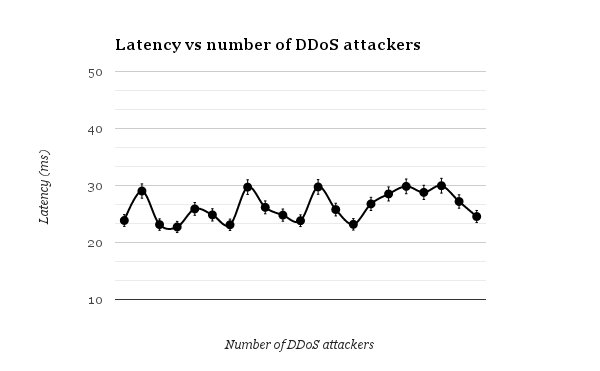
\includegraphics[width=16cm]{latency.png}
\end{center}
\caption{Variation in latency w.r.t. scaling DDoS attack}
\label{fig:latency}
\end{figure*}

We carried out our evaluation scaling from 0 to 20 DDoS attacker nodes a total of 10 times and averaged the results. We found that service latency is nearly constant with respect to the scale of the DDoS attack. In particular, we found a mean latency of $\mu\approx 26.26\mbox{~ms}$ and standard deviation $\sigma\approx 2.57\mbox{~ms}$. This result is summarized in Figure~\ref{fig:latency}.

Additionally, of the total of 521 legitimate requests sent manually to the system, we found that 508 of the requests were responded to (97.5\%). That is, only 2.49\% of requests were mis-classified as malicious and dropped.


\section{Conclusion}

Distributed denial of service attacks prove very difficult to recognize and mitigate, as they are indistinguishable from normal traffic except in the volume of activity. Our system aims to exploit this single characteristic to classify and withstand such attacks.   We perform a cluster-based analysis of request times and classify sources based on their appearance during DDoS attacks. With this system, we are able to quickly and efficiently classify sources, resulting in effectively constant service latency in the face of a DDoS attack while dropping a minimal number of legitimate user packets.

\section{Acknowledgements}

We would like to thank Prof. Hakim Weatherspoon and Erluo Li for providing feedback and suggestions.

\bibliography{paper}{}
\bibliographystyle{plain}

\end{document}
